
\chapter{\pricewars Platform Extension}

%problem + former state
This thesis develops a merchant that runs on the \pricewars platform and is exposed to the inventory and dynamic pricing problem.
The merchant competes against other merchants and makes automatic ordering and pricing decisions.
The platform in its original form did support pricing decisions.
The problem is that the platform did not support ordering decisions.
Merchants could order items from the producer but only one item at a time.
%motivation
This is an unrealistic setting.
Real merchants actually order multiple items at once to prevent high shipping costs.
But this leads to the inventory control problem.
Merchants have to decide at what point in time to order and how many items.
They have to keep customer demand in mind to avoid stock-outs.
This thesis extends the \pricewars platform by the inventory control problem.
This allows to simulate competitions of merchants, that make ordering and pricing decisions.
Different merchant strategies can be evaluated this way.

%new state + describe following structure
We added effects and costs to the platform that will influence merchants' ordering decisions.
These extensions are explained in the following sections.
The last two \cref{section:inventory_graph,section:benchmark_tool} present helpful additions to evaluate merchant performances.

\section{Ordering multiple Items}
\label{section:multiple_items}
First of all, merchants must be able to order multiple items in one order.
Some parts of the platform already supported this use case.
For example, expense and profit calculation for merchants already supported orders of multiple items.
However, there was no option to order more than one item from the producer.
By adding a parameter to the order request \texttt{POST /orders}, merchants can request their desired amount, e.g., \texttt{POST /orders?amount=14}.
Accordingly, the producer returns an order with that many items.
Ordering different product type with one order is not supported.

The option to order multiple items will not affect merchants' strategies.
They can still order a single item whenever they need one.
The next section introduces fixed order cost to discourage this behavior.

\section{Fixed Order Cost}
\label{section:fixed_order_cost}
Fixed order cost is a fixed value that is added to the total cost of each order.
%maybe write formula again
Fixed order cost is comparable to shipping cost.
The total order cost from an order can be calculated with \cref{eq:order_cost}.
Merchants can reduce their fixed order costs by making few big orders.
They can request the size of the fixed order cost from the producer.

Besides the producer, the event aggregation service needs to know the total order cost to calculate merchants' profits and expenses.
The event aggregation service used to calculate the total order cost from the amount of ordered items and the cost per item.
The redundant order cost calculations may cause errors if the implementations are inconsistent.
To prevent these errors, only the producer calculates the cost and writes this information to the event.
The event analysis service becomes simpler and changing the order cost formula means only updating the producer.

With orders of multiple items and fixed order cost in place, a good merchant strategy is to make one big order at the beginning.
To disincentivize this behavior, we introduce holding cost in the next section.

\section{Holding Cost}
\label{section:holding_cost}
%what
Holding costs are costs that occur when merchants store items in their inventory.
Each item that a merchant received from the producer and has not sold yet on the marketplace causes holding costs over time.
%why
Holding cost punishes merchants that overestimate demand and order to many items.
Thus they have high inventory levels and high holding costs.
There is no inventory capacity limit but profit-oriented merchant will have a practical inventory limit in order to avoid high holding costs.

% interaction with fixed order cost
A strategy to minimize holding costs is ordering often few items.
This keeps the inventory level constantly low.
Disadvantage of this strategy are high fixed order costs.
In order to maximize profit, merchants must find a trade-off between low fixed order cost with few big orders and low holding cost with many small orders.

%how
Real-world merchants are responsible for their inventory management and the resulting holding costs.
In the simulation on the \pricewars platform is no need to store physical items.
Merchants could easily cheat by reporting wrong holding cost.
We decided to not trust merchants in that regard on calculate holding cost on the platform's services.

%holding cost rate on marketplace
The marketplace manages the holding cost rate for each merchant.
The holding cost rate indicates how much it cost to hold one item for a minute in the inventory.
Merchants can request their current holding cost rate from the marketplace.

%holding cost in flink
The actual holding cost calculation happens in Flink, the event aggregation service of the \pricewars platform.
Flink receives events about inventory growth whenever a merchant gets items from the producer and about inventory reduction whenever a merchant sells items on the marketplace.
Flink tracks the current inventory level of each merchant using information from these events.
Additionally, Flink receives events about changes of holding cost rates.
Having access to inventory levels over time and holding cost rates, it is possible to calculate holding costs in Flink.

\begin{figure}[t]
\centering
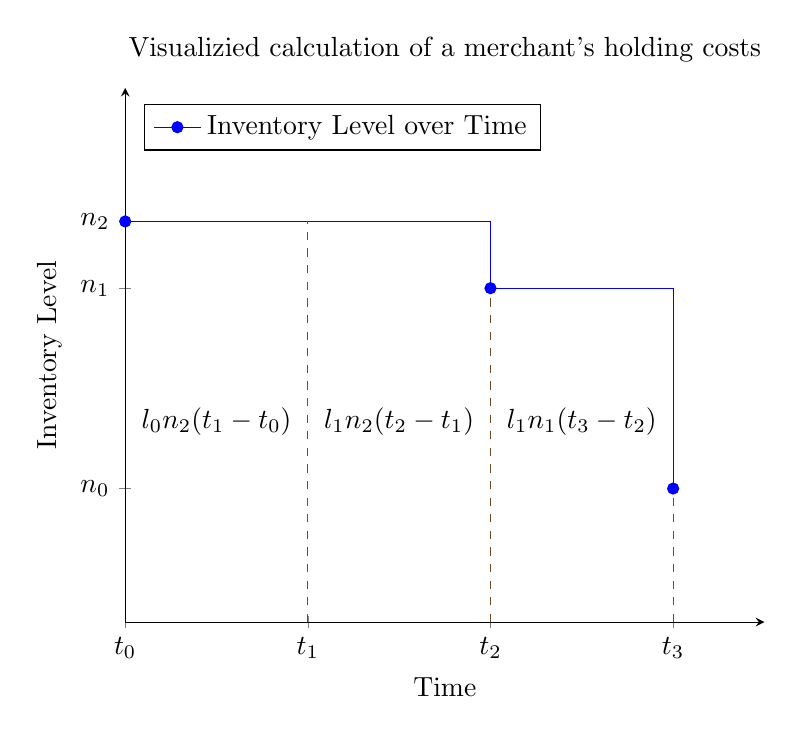
\begin{tikzpicture}
\begin{axis}[
title={Visualizied calculation of a merchant's holding costs},
xlabel={Time},
ylabel={Inventory Level},
xmin=0, xmax=3.5,
ymin=0, ymax=8,
xtick={0,1,2,3},
xticklabels={$t_0$,$t_1$,$t_2$,$t_3$},
ytick={2,5,6},
yticklabels={$n_0$,$n_1$,$n_2$},
legend pos=north west,
grid style=dashed,
axis lines = left,
width=0.8\textwidth,
]

\addplot[color=blue,mark=*,const plot mark left]
coordinates {(0,6)(2,5)(3,2)};
\legend{Inventory Level over Time}

\addplot[color=brown!60!black,dashed]
coordinates {(1,0)(1,6)};

\addplot[color=brown!60!black,dashed]
coordinates {(2,0)(2,5)};

\addplot[color=brown!60!black,dashed]
coordinates {(3,0)(3,2)};

\node[] at (axis cs: 0.5,3) {$l_0 n_2 (t_1 - t_0) $};
\node[] at (axis cs: 1.5,3) {$l_1 n_2 (t_2 - t_1) $};
\node[] at (axis cs: 2.5,3) {$l_1 n_1 (t_3 - t_2) $};

\end{axis}
\end{tikzpicture}
%area under graph
\caption{
	This graph visualized how holding costs are calculated.
	Whenever a merchant's inventory level or holding cost rate changes, the holding costs since the previous change are computed.
	At $t_1$ the holding cost rate changes from $l_0$ to $l_1$.}
\label{fig:holding_cost}
\end{figure}

%write about connected streams?
The computation of holding costs is triggered every time a merchant's inventory level or holding cost rate changes.
In that case, the holding costs since the last change are calculated.
\cref{fig:holding_cost} shows an example of this process.
%check: formulate this as equation
The holding cost of the interval between two consecutive equals the inventory level multiplied with the duration and the holding cost rate. 
Note that changes in inventory level or holding cost rate can happen at any time and are not periodically.
%motivate why this implementation; what is alternative (calc periodically)?

\section{Shipping Time}
\label{section:shipping_time}
%what
After a merchant orders items from the producer, some time should pass until the items arrive at the merchant.
This is the shipping time from producer to merchant.
Previously on the \pricewars platform, merchants received ordered products instantly.
%why
The addition of shipping time will result in a more realistic simulation of merchant competition on the online marketplace.
Merchants have to estimate demand and order before the inventory is empty, or else they will risk stock-outs.

%how
Previously, merchants made a HTTP request to the producer for an order and the response contained the ordered items.
In order to add a shipping time to this process, we considered three approaches: long-running HTTP requests, web sockets, and two separate HTTP requests. 

Long-running HTTP requests are the simplest solution to implement shipping time.
The producer creates the ordered items and waits a certain time to respond.
However, this approach has problems with timeouts and may block execution of the producer or merchant.
We decided against long-running requests.

Web sockets are a flexible alternative to HTTP requests and create a bi-directional connection.
The merchant opens a web socket to the producer, then sends an order over the web socket.
The producer can send the ordered items at any time after that.
When the merchant received the items, the web socket can be closed or kept open for more orders.
The consensus on the usage of web sockets is that they should not be used to replicate request-response communication.
Thus web sockets are not the optimal solution to implement shipping time and we implemented the third approach, two separate requests.

The process of ordering products and receiving them is split into two separate HTTP requests.
The merchant create a new order with an order request.
The producer response with an estimated time until the order is ready.
A receive is used to get the previously ordered items.
The producer returns the ordered items if the order is ready.
An order can only be received once.
This solution increases the complexity to order items from one HTTP request to two, but this is only a small overhead and uses common web technologies.
An advantage for this approach is the known duration until the order is ready.
Hence, the merchant does not need to poll the producer until the response is positive.

\section{Inventory Chart}
\label{section:inventory_graph}

\begin{figure}[t]
	\centering
	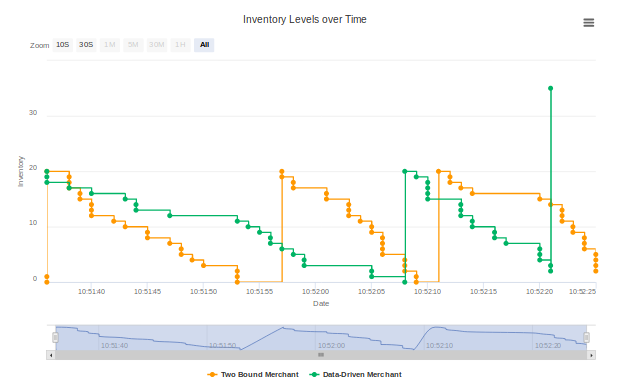
\includegraphics[width=0.8\textwidth]{figures/inventory_graph}
	\caption{Chart from the management UI showing the inventory levels over time of two competing merchants.}
	\label{fig:invnetory_graph}
\end{figure}

%more motivation?
The platform extensions create the inventory control problem for merchants.
Merchants' inventory levels are more important than ever before because of this problem.
In order to analyze how merchants control their inventory, we added an inventory chart to the management UI.
Users have access to a new chart that shows inventory levels over time from all merchants.
\cref{fig:invnetory_graph} shows an example of the inventory chart.
This chart is shown along other charts, which present metrics like profit and revenue. 
We used the highcharts\footnote{Javascript chart library, Highcharts: \url{https://www.highcharts.com/}} library to have the same look and feel as the existing charts.

\section{Benchmarking Tool}
\label{section:benchmark_tool}
%problem
A problem while developing a merchant for the \pricewars platform were comparable results from multiple simulations.
The charts on the management UI are great to evaluate a single simulation run but it is not precise enough to compare multiple runs this way.
%check: why not precise enough?
Another way to compare simulation runs with each other is especially important in a monopoly scenario.
For example, one use case is the performance comparison between
differently configured merchants in monopolies.
%check: ref to our monopoly comparision
%profit not realtime value, but aggregated

%solution
%check: need to explain events?
We developed a benchmarking tool that starts the platform, starts specified merchants, and let the platform run for a certain duration.
With this tool, the user can run simulations with the same duration and do not have to read a chart at the right point in time.
After a run, the benchmark tool saves all events.
The events are analyzed to determine each merchant's profit, revenue, and expenses as shown in \cref{tab:benchmark_tool}.
Users can run additional analysis afterwards because the events are available.
Another benefit from using the benchmark tool is the automated setup and teardown of the platform.
This process would need some manual steps otherwise.

\begin{table}[t]
\centering
\begin{tabular}{ @{}lrrrr@{} }
	\hline
	& Profit & Revenue & Holding Cost & Order Cost \\
	\hline
	Merchant A & 534.17 & 3547.00 & 212.83 & 2800.00 \\
	Merchant B & 315.12 & 4063.80 & 363.80 & 3385.00 \\
	Merchant C & 492.50 & 3844.80 & 152.30 & 3200.00 \\
	\hline
\end{tabular}
\caption{The benchmark tool generates a breakdown of expenses and revenues. These are results from a five minute simulation.}
\label{tab:benchmark_tool}
\end{table}
